\section{Bicycle Station}
The station software package contains two aspects, software intended to be run on the stations that are placed at each bicycle location throughout the city, and software to simulate the hardware we do not have access to, used as proof of concept.

\subsection{Station Software}
The station software contains three parts.
A listener that listens for signals from the global database interface, signalling that a booking has been created or removed.
A lock manager that is responsible for locking a dock when a booking is close to its start time, and unlocking if a booking has expired.
Communication with the global Database through a SOAP service interface described in \secref{sec:webToStationI}.

\textbf{Listener}
The listener is made as a Tcp Listener based heavily on code found on Microsofts Developer Network\citep{misc:TcpListenerSource}. 
The listener listens for messages reporting changes in bookings, either addition of a booking or removal of one. 
The messages are JSON encoded strings of two different forms depending on the content which can be seen in \lstref{lst:JsonUnbooking} and \lstref{lst:JsonBooking}.

\begin{minipage}{\textwidth}
\begin{minipage}{0.45\textwidth}
\begin{lstlisting}[caption = {Example of an unbooking message}, label = {lst:JsonUnbooking}]
{
 "action":"unbooking",
 "start_station":5,
 "booking_id":2
}
\end{lstlisting}
\end{minipage}
\hspace{0.5cm}
\begin{minipage}{0.45\textwidth}
\begin{lstlisting}[caption = {Example of a booking message}, label = {lst:JsonBooking}]
{
 "action":"booking",
 "start_station":5,
 "booking_id":2,
 "start_time":1414135298,
 "password":483923
 }
\end{lstlisting}
\end{minipage}
\end{minipage}

The information contained in the received message is then used to either remove a booking from the database, or add a booking to the database at the specified station, which type is decided based on the action parameter.

\textbf{SOAP Service}
%-communication with global DB
The SOAP Service is used to report changes in the data relevant to the global database, which is

\begin{itemize}
\item Booking used
\item Booking expired
\item Bicycle taken from station
\item Bicycle returned to station
\end{itemize}

There is also a fifth use at the start of the program.
This is done only once and is used to refresh the bookings in the station database after a system reboot, where all bookings are first removed from the station database, and then all bookings are requested from the global database through the interface.

\textbf{Lock Manager}
The \textit{LockManager} runs in its own thread, with the sole responsibility of locking and unlocking docks based on booking start times. 
Currently the time constraints is set to locking a bicycle to a dock one hour before booking start time, and unlocking again 1 hour after start time. 
As this functionality requires constant monitoring, the function is run in an infinite thread, however, since we do not want to waste our processor time by executing this constantly, it sleeps at the end of its execution loop for a minute. 
A minute sleep time is deemed appropriate as the data is not rapidly changing and faster responses are not necessary.

The loop starts out by finding all the expired bookings, removing the lock they had on a bicycle, telling the global database that the bookings have expired, and removing the bookings from the station database.
The loop then finds all bookings that start within the next hour, and, if any of these bookings were not locked in the last iteration of the loop, locks a bicycle for the booking.

At the end of the execution of the loop the UI is updated to reflect any changes performed to the database.


\textbf{Graphical User Interface}
The Main UI window has two parts, which can be seen in \figref{fig:stationMain}, part one is the station software, and part two is for the hardware simulation.

\begin{figure}
	\centering
	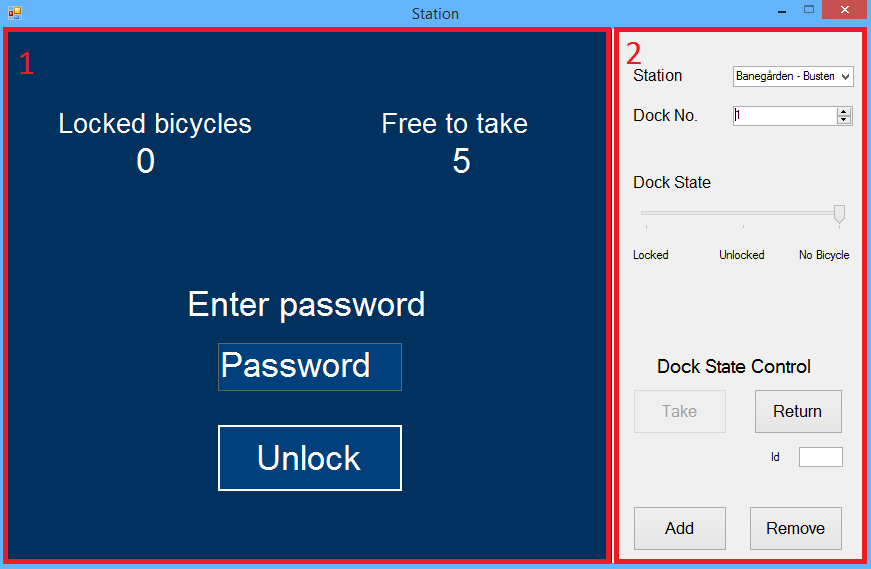
\includegraphics[scale=0.4]{stationsoftware/mainwindow}
	\caption{UI for the station software}\label{fig:stationMain}
\end{figure}

The station software UI, part 1 in \figref{fig:stationMain}, has been designed to be simple and understandable by users of the system with only the necessary content.
The blue colour was chosen as this is the colour of the bicycles and the \bycykel homepage.
The station software UI is divided into two pages, the first one can be seen in the figure.
It has a field to input a password for a booking to unlock the booked bicycle.
In addition to this it also displays how many bicycles on the station that are locked and how many that are free to take.
When a valid booking password is input, the station software changes, which can be seen in figure \figref{fig:bicycleUnlock}.
The user is told at which dock the bicycle for him/her has just been unlocked.
There is also a button to quickly return to the main window, which otherwise happens after two minutes.

\begin{figure}
	\centering
	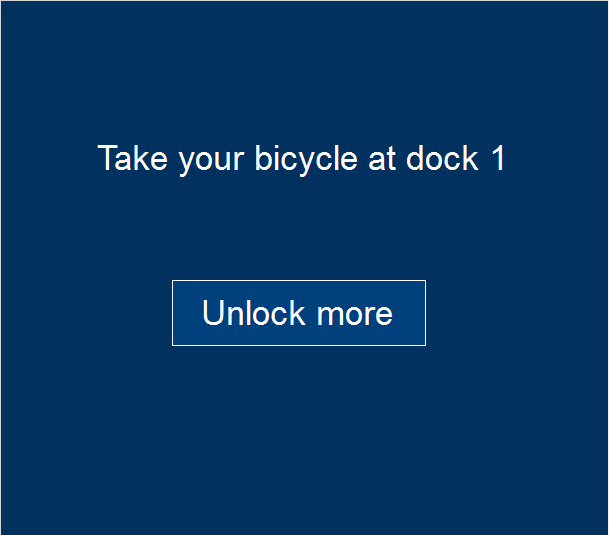
\includegraphics[scale=0.4]{stationsoftware/unlockwindow}
	\caption{UI for unlocked bicycle}\label{fig:bicycleUnlock}
\end{figure}

\textbf{Simulation of Hardware}
The part of the UI representing the simulated hardware is the second part seen in \figref{fig:stationMain}.
The simulated hardware represents what would normally be observed at the physical station.
We simulate the ID chips on the bicycles and the lock on the dock.
The ID chips are simulated when they would normally have been read at the docks, which is when the bicycles are returned to it after use.
In this case, when a bicycle is returned, we find a random ID from among those not currently in a dock, and selects this as the ID returned.
Random ID is sufficient at this time, as we have no way of predicting where a bicycle in use would be returned to.
The lock is simulated by a boolean representation, stating if it is locked or not.

In the simulation part of the UI, there is a dropdown list where it is possible to select which station a user is standing at, along with a numeric selector allowing selection of a specific dock at the current station.
In addition, there is also a slide bar showing the state of the selected dock.
The possible states being locked, unlocked and no bicycle.
At the bottom of the UI there are two buttons that simulate the user actions of returning and removing a bicycle.

\subsubsection{Data Loss}
With the communication between the station software and the global database, there is a risk of losing data during the communication or not having a connection at all.
The case of lost data is currently unhandled, which results in the system entering an unstable state where it is likely to not behave as expected. 
\fxwarning{Update when something  is done about these issues}